\documentclass{standalone}
\usepackage{tikz}
\usetikzlibrary{automata, positioning, arrows}

\begin{document}
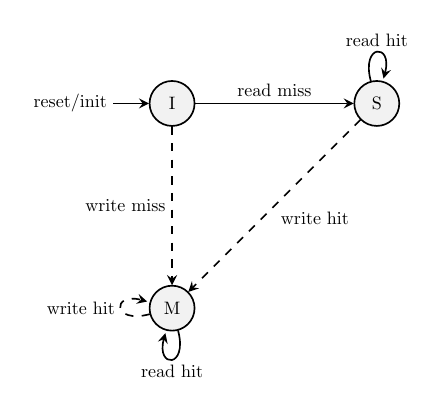
\begin{tikzpicture}[node distance=4cm,initial text={reset/init}]
\tikzstyle{every node}=[scale=0.65]
\tikzstyle{every state}=[semithick, fill=gray!10]
\tikzstyle{every edge}=[draw,->,>=stealth,auto,semithick]

\node[state] (M) {M};
\node[state, above of=M,initial] (I) {I};
\node[state, right of=I] (S) {S};

\draw (M) edge[loop below] node {read hit} (M)
            edge[loop left, dashed] node {write hit} (M);
\draw (I) edge[dashed] node[left] {write miss} (M)
            edge node {read miss} (S);
\draw (S) edge[dashed] node {write hit} (M)
            edge[loop above] node {read hit} (S);
\end{tikzpicture}
\end{document}
